\documentclass[a4paper,twoside,12pt,openright]{report}

%% Language %%%%%%%%%%%%%%%%%%%%%%%%%%%%%%%%%%%%%%%%%%%%%%%%%
\usepackage[francais]{babel}
\usepackage[utf8]{inputenc}
\usepackage[T1]{fontenc}
\usepackage{lmodern} 
\usepackage{hyperref}
\usepackage{tabto}
\usepackage{xcolor}
\usepackage{sectsty}
\definecolor{couleur}{RGB}{255,0,0}
\definecolor{couleur2}{RGB}{200,0,0}
\chapterfont{\color{couleur}}
\sectionfont{\color{couleur}}
\subsectionfont{\color{couleur2}}

%% Packages for Graphics & Figures %%%%%%%%%%%%%%%%%%%%%%%%%%
\usepackage{graphicx} 

%% Math Packages %%%%%%%%%%%%%%%%%%%%%%%%%%%%%%%%%%%%%%%%%%%%
\usepackage{amsmath}
\usepackage{amsthm}
\usepackage{amsfonts}
\usepackage{fullpage}

\setlength{\parindent}{0cm}
\setlength{\parskip}{1ex plus 0.5ex minus 0.2ex}
\newcommand{\hsp}{\hspace{20pt}}
\newcommand{\HRule}{\rule{\linewidth}{0.5mm}}
%%%%%%%%%%%%%%%%%%%%%%%%%%%%%%%%%%%%%%%%%%%%%%%%%%%%%%%%%%%%%
%% DOCUMENT
%%%%%%%%%%%%%%%%%%%%%%%%%%%%%%%%%%%%%%%%%%%%%%%%%%%%%%%%%%%%%
\begin{document}
\begin{titlepage}
  \begin{sffamily}
  \begin{center}

    \textsc{\LARGE MASTER MIAGE 2ème année \linebreak Université Paris Nanterre}\\[2cm]

    \textsc{\Large Mémoire de fin d’études présenté pour l’obtention du grade de master}\\[1.5cm]

    \HRule \\[0.4cm]
    { \huge \bfseries Comment les flots de contrôle peuvent nous permettre de faire du refactoring de code en Java. \\[0.4cm] }

    \HRule \\[2cm]
    
\includegraphics[scale=0.40]{image/univ.jpg}
    \hspace{2cm}
    
    \vfill
  \begin{minipage}{0.4\textwidth}
      \begin{flushleft} \large
        \textsc{Présenté par :}\\ \textsc{Thibault Sartre}\\
      \end{flushleft}
    \end{minipage}
    \begin{minipage}{0.4\textwidth}
      \begin{flushright} \large
        \textsc{Tuteur :}\\ \textsc{Mcf. Emmanuel Hyon}\\
      \end{flushright}
    \end{minipage}
    \vfill
    {\large Septembre 2018 — Juin 2019}
  \end{center}
  \end{sffamily}
\end{titlepage}
\renewcommand{\contentsname}{Sommaire}
\tableofcontents{}



\chapter{Introduction}

\section{Remerciements}
Je tiens à remercier les professeurs de l'université de Paris Nanterre pour m'avoir suivi pendant ces deux dernières années de master.\\
J'aimerais aussi remercier Emmanuel Hyon mon tuteur pour sa disponibilité et son aide lors de la réalisation de ce mémoire.\\


\section{Introduction}
Le refactoring est une activité d'ingénierie logicielle consistant à modifier le code source d'une application de manière à améliorer sa qualité sans altérer son comportement vis-à-vis des utilisateurs.
L'objectif du refactoring est de réduire les coûts de maintenance et de pérenniser les investissements tout au long du cycle de vie du logiciel en se concentrant sur la maintenabilité et l'évolutivité.\cite{ref1}\\
"With refactoring you can take a bad design, chaos even, and rework it into well-designed code."\cite{ref2}\\
Le refactoring permet donc de passer d'un code possédant de mauvaises bases à un code propre.\\
Un bon refactoring doit pouvoir améliorer la qualité d'un code tout en gardant son fonctionnement du point de vue de l'utilisateur. Concernant la partie des tests, tous les tests qui fonctionnaient avant le refactoring se doivent d'être fonctionnels après.\\
Dans ce mémoire, nous allons d'abord étudier les problèmes dans les programmes qui mènent au refactoring. Ensuite on va analyser différentes techniques de refactoring. Enfin nous allons étudier les outils de refactoring existant ainsi que les graphes de flots de contrôle et s'ils sont utilisables dans le refactoring.\\
Le plan de ce mémoire a été élaboré à l'aide de plusieurs sources (\cite{ref3},\cite{ref4},\cite{ref5},\cite{ref8},\cite{ref14},\cite{ref7}).\\
Ce sujet est intéressant et actuel car il faut commencer à se soucier du code que l'on produit car plus l'on avance dans le temps plus les programmes sont lourds et contiennent de lignes de code. Avec la puissance des ordinateurs actuels, la plupart des développeurs ne prennent plus le temps d'écrire des codes de qualité car la machine sera de toute façon assez rapide pour compenser un code de mauvaise qualité.\cite{ref4}\\
A l'avenir, la relecture et la modification de code seront plus difficiles, avec les programmes devenant de plus en plus gros.\cite{ref4}\\
Pour essayer de diminuer cette quantité de travail, il faut commencer à produire du code de qualité et bien structuré. Concernant les codes déjà existants il faudra donc faire du refactoring de code. Or le refactoring peut être long selon la qualité des projets que l'on traite. Il serait donc intéressant et très utile d'avoir un programme permettant d'automatiser des parties de refactoring pour permettre de gagner un temps précieux. 
Ce mémoire a pour but d'établir s'il est possible de faire du refactoring à l'aide des graphes de flots de contrôle.\cite{ref3}\\
Lien github vers le dépôt du mémoire: "https://github.com/ThibaultSartre/MemoireM2"\\

\chapter{Pourquoi faire du refactoring ?}
\section{Bloaters}
Les bloaters (ou ballonnements) peuvent être des classes, des méthodes ou même du simple code qui ont pris des proportions énormes, ce qui rend le travail  compliqué. Si on n'y prend pas garde, ce type de problème se développe au fil du temps.\\

\subsection{Méthode trop longue}
\paragraph{Problème :}
Un des soucis que beaucoup de développeurs rencontrent, est qu'ils préfèrent rajouter des lignes de code dans une méthode existante plutôt que de créer une nouvelle méthode sous prétexte que cette nouvelle méthode ne ferait que quelques lignes.\\
Cela engrange des méthodes trop grosses et difficiles à lire et à maintenir.\\

\paragraph{Gain du traitement :}
Le refactoring d'une méthode trop longue permet à cette même méthode de vivre plus longtemps du fait de sa simplicité.\\
Cela permet aussi en général de supprimer potentiellement une duplication de code.\\
Avec une méthode qui est maintenant petite et claire, il est alors beaucoup plus simple et rapide de la maintenir.\\

\subsection{Grande classe}
\paragraph{Problème :}
Comme pour la méthode trop longue, on a tendance à préférer placer une nouvelle fonctionnalité dans une classe existante plutôt que de créer une nouvelle classe.\\
Ce qui en découle est une classe monstrueusement grande, ce qui la rend très difficilement praticable.\\

\paragraph{Gain du traitement :}
Une fois le refactoring effectué, le développeur n'a plus à avoir en tête les dizaines et dizaines d'attributs et méthodes qui composent sa classe.\\
Et comme dit précédemment le découpage d'une classe va aussi en général permettre une suppression de doublon de code ou au moins le rendre moins apte à apparaître.\\

\subsection{L'obsession des types primitifs}
\paragraph{Problème :}
Les problèmes liés aux types primitifs sont :\\
- l'utilisation d'un simple type "string" pour un numéro de téléphone ou bien un "integer" pour représenter un montant d'argent à la place d'objet.\\
- l'utilisation de constantes pour coder de l'information comme des droits administrateurs\\
- l'utilisation de chaînes de caractères en guise de noms de champs dans des tableaux de données.\\

\paragraph{Gain du traitement :}
On obtient un code plus flexible grâce à l'utilisation d'objet.\\
Plus besoin de se demander à quoi servent toutes ces constantes.\\
Globalement le code est plus compréhensible.\\

\subsection{Longue liste de paramètres}
\paragraph{Problème :}
On peut considérer qu'une liste de paramètres devient trop longue dès lors qu'elle contient plus de quatre paramètres.\\
Une longue liste de paramètres peut vouloir dire qu'une méthode est en fait la combinaison de plusieurs.\\
Ces listes sont difficiles à comprendre; il est préférable d'utiliser les attributs de la classe où se trouve la méthode. Et si ce n'est pas possible il est préférable d'envoyer un objet qui regroupe les données nécessaires.\\

\paragraph{Gain du traitement :}
Le code devient plus lisible.\\
Il peut être raccourci dans le cas où la méthode est une fusion de plusieurs.\\

\subsection{Agrégat de données}
\paragraph{Problème :}
Parfois il est possible de trouver des groupes de variables identiques qui apparaissent à plusieurs endroits dans le code.\\
Ces agrégats sont souvent dûs à de la programmation "copié collé" ou à une structure pauvre du programme.\\
Pour savoir s'il est possible d'extraire ces agrégats de données pour former une nouvelle classe, il faut vérifier si c'est bien le groupement de toutes ces données qui leur donne du sens (par exemple les données nécessaires à la connection vers une base). Si c'est le cas, le choix de créer une nouvelle classe pour ces données est conseillé.\\

\paragraph{Gain du traitement :}
Permet de faciliter la compréhension et l'organisation du code et surtout de ses agrégats de données puisque les opérations liées à ces données sont maintenant regroupées vers une seule classe.\\

\section{Abus du principe orientation objet}
Il s'agit de problème basé sur la mauvaise utilisation du principe de programmation "orienté objet".\\

\subsection{La structure switch}
\paragraph{Problème :}
Ce problème survient lorsque l'on obtient un "switch" ou une séquence de "if" complexe.\\
Les "switch" de ce type peuvent être utilisés pour faire un traitement différent selon le type d'un objet.\\
Par exemple, on a une classe Oiseau qui possède une méthode getSpeed(). Cette méthode va , à l'aide d'un switch, analyser un attribut qui définit quel oiseau représente la classe pour renvoyer la vitesse de cet oiseau.\\
Dans ces cas là, il est préférable d'utiliser le polymorphisme (voir \textit{Remplacer les conditions avec du polymorphisme}).

\paragraph{Gain du traitement :}
On obtient une meilleure organisation du code.\\

\subsection{Héritage refusé}
\paragraph{Problème :}
Ici, le problème survient lorsque l'on commence à créer des sous-classes uniquement pour ré-utiliser certaines méthodes de la super classe alors que la super classe et la sous classe ne possèdent pas de réel lien.\\


\paragraph{Gain du traitement :}
En supprimant ces liens entre les classes, on obtient  un code plus organisé et clair.\\
On n'aura plus d'héritages "bizarres" qui n'ont aucun sens.\\

\section{Modification complexe}
Dans cette section, nous allons parler de problèmes liés à la modification difficile de code.\\
Par exemple lorsqu'on doit modifier du code à différents endroits pour faire fonctionner le tout.\\

\subsection{Changement Divergent}
\paragraph{Problème :}
Ce problème cible particulièrement le cas où un simple changement dans une classe produit un grand nombre de changements dans d'autres méthodes de cette même classe.\\
Par exemple dans le cas d'une classe produit, où l'on veut rajouter un type de produit, il faut alors changer les méthodes de recherche, d'affichage et d'ordonnancement de produit.\\
Pour cet exemple, il faudrait utiliser la technique de refactoring d'extraction de classe.\\

\paragraph{Gain du traitement :}
Avec ce traitement, on simplifie la maintenance du code et on simplifie son organisation.\\

\subsection{Chirurgie au fusil}
\paragraph{Problème :}
Cette fois, on a un problème totalement inverse au précédent, c'est à dire qu'ici un petit changement demande de faire des petits changements dans plusieurs classes.\\
On a ce problème dans le cas où une responsabilité de traitement est affectée à plusieurs classes et si ce traitement doit changer, toutes les classes doivent être modifiées.\\
Les refactoring utilisés pour réparer le code sont le "déplacement de méthode et d'attribut".\\

\paragraph{Gain du traitement :}
En revanche les avantages du traitement sont les mêmes que précédemment c'est à dire une meilleure organisation et une maintenance simplifiée.\\

\newpage

\section{Les choses dispensables}
Dans cette partie, nous allons parler de toutes les petites choses qui sont dans le code mais qui ne servent à rien.

\subsection{Les commentaires}
\paragraph{Problème :}
Attention je ne dis pas que les commentaires en général sont inutiles.\\
Il y a problème lorsque on utilise les commentaires pour masquer un code d'une qualité douteuse.\\
Dans ce cas précis, les développeurs vont écrire du code très peu compréhensible au premier regard et le remplir de commentaires afin de tout expliquer.\\
Pour remédier à ce problème, on va suivre la règle : "Le meilleur des commentaires est un bon nom de méthode, classe ou variable".\\

\paragraph{Gain du traitement :}
En renommant nos méthodes, classes et variables pour que leurs noms représentent ce qu'elles contiennent ou font, on obtient un code avec beaucoup moins de commentaires mais qui devient bien plus intuitif et facile à comprendre.\\
Les commentaires restants ne sont plus là pour expliquer ce que contient une variable avec un nom peu évocateur tel que les variables temporaires qui s'appellent "tmp".\\

\subsection{La duplication de code}
\paragraph{Problème :}
Ce problème peut arriver lorsque plusieurs développeurs travaillent en même temps sur le même projet. Ainsi une fonctionnalité sera développée deux fois à deux endroits différents du code.\\
La duplication de code entraîne une réécriture plus longue de la fonctionnalité dupliquée car il faut la modifier à plusieurs endroits du code, et il est aussi possible d'oublier de modifier la fonctionnalité dans une des parties.\\
Pour supprimer la duplication de code il est conseillé d'utiliser la technique de refactoring "Extraction de méthode" qui va permettre d'extraire la méthode pour ensuite uniquement faire des appels de méthodes.\\

\paragraph{Gain du traitement :}
La suppression de la duplication de code nous permet de réduire la taille du code et donc de le simplifier, ce qui rend le code plus facile à modifier et faire évoluer.\\

\subsection{Les classes paresseuses}
\paragraph{Problème :}
La maintenance et la compréhension d'une classe sont des choses qui prennent du temps. Il est donc judicieux de faire en sorte de ne pas garder des classes qui ne sont plus pertinentes et qui font perdre plus de temps qu'elles ne sont utiles.\\
Ici nous allons parler d'une classe qui ne contient que très peu de fonctionnalités et qui est devenue très petite avec le temps suite à d'autres refactorings.\\


Ce type de classe n'a plus grand intérêt; il est donc intéressant de déplacer le peu de fonctionnalités restantes de la classe vers une autre classe puis de la supprimer.\\

\paragraph{Gain du refactoring :}
Supprimer des classes peu utiles voir inutiles permet de réduire la taille du code et de faciliter sa compréhension et sa maintenance.\\

\subsection{Les classes de données}
\paragraph{Problème :}
Une classe de données est une classe qui contient un regroupement de données qui permettent de faire des traitements si elles sont regroupées.\\
Ces classes de données sont utiles mais peuvent rapidement perdre de leur utilité lorsqu'elles sont utilisées uniquement comme un stockage de données. C'est à dire que la classe de données ne contient pas de fonctionnalité et ne contient que les variables avec des getters et setters.\\
Il est donc préférable de regrouper toutes les fonctionnalités liées à cette classe de données éparpillées dans tout le code pour les insérer comme des méthodes de la classe de données.\\ 

\paragraph{Gain du traitement :}
Regrouper les fonctionnalités va permettre de supprimer d'éventuelles  duplications de code.\\
Et cela permet surtout de faciliter la maintenance du code puisque toutes les fonctionnalités liées aux données sont regroupées dans la même classe.\\

\subsection{Le code mort}
\paragraph{Problème :}
Un code mort est un bout de code qui n'a plus aucune utilité à l'instant T. Il peut s'agir de n'importe quoi, une classe, une variable, une méthode ou même un paramètre.
Une personne qui reprend du code ne va pas savoir que ce code n'a plus de raison d'exister et risque de perdre du temps en essayant de comprendre son utilité.\\

On peut aussi générer du code mort lorsque l'on développe de manière prévisionnelle : on pense que dans le futur on aura besoin de cette fonctionnalité.
On développe donc certaines fonctionnalités juste au cas où on en ait besoin.\\
De ce fait, la fonctionnalité n'a jamais été utilisée et on se retrouve avec du code mort.\\

La meilleure chose à faire avec du code mort c'est de le supprimer.\\

\paragraph{Gain du traitement :}
Supprimer du code mort permet de réduire la taille du code considérablement selon ce qui est supprimé mais aussi cela va rendre le code beaucoup plus simple à maintenir.\\




\chapter{Les différents types de refactoring}
Dans ce chapitre, je vais vous présenter des méthodes de refactoring qui permettent d'améliorer la qualité du code.\\

\section{Pattern de méthode composée}
Une méthode trop longue et peu compréhensible est difficile à maintenir pour un développeur.
Une grande partie du refactoring est donc consacrée à la composition correcte des méthodes.\cite{ref5}\\

L'objectif de ce type de refactoring est de :\\
- rendre les méthodes facilement compréhensibles.\\
- simplifier les méthodes en les brisant en plusieurs méthodes plus petites.\\
- supprimer la duplication de code.\\
- nommer proprement les variables, méthodes et paramètres pour comprendre leurs utilités au premier coup d'œil.\\
- pouvoir faire des tests plus facilement car les morceaux de méthodes peuvent être testés individuellement.\cite{ref6}

\newpage

\subsection{Extraction de méthode}
\paragraph{Présentation :} 
La technique d'extraction de méthode permet, comme son nom l'indique, d'extraire des méthodes (ou fonctions) du code. Car plus il y a de lignes dans une méthode plus il est difficile de comprendre ce que fait la méthode.\\
Il faut donc lorsque c'est possible extraire du code pour former d'autres méthodes et simplifier le code.
\begin{center}
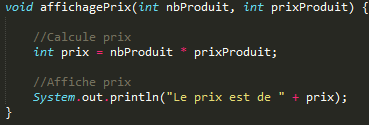
\includegraphics[scale=1]{Image/Extraction_Methode.png}\\
\itshape{Avant extraction de méthode}
\end{center}

\paragraph{Exemple :} 
Ci-dessus nous avons une méthode qui va afficher le prix d'un produit tout en calculant elle-même le prix.\\
Si l'on applique l'extraction de méthode, on va obtenir l'exemple du bas, c'est à dire extraire la méthode de calcul du prix car on en aura sûrement besoin ailleurs. On remplace donc le calcul du prix dans la méthode affichagePrix par un appel à la méthode calculePrix.\\
\begin{center}
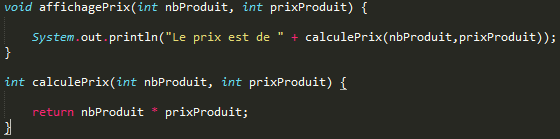
\includegraphics[scale=1]{Image/Extraction_Methode2.png}\\
\itshape{Après extraction de méthode}
\end{center}
\paragraph{Bénéfices :}
Pour que cette technique de refactoring soit la plus efficace, il faut absolument nommer ses méthodes et les paramètres de manière à comprendre très facilement quel est son but et que représentent les paramètres. Le code est donc bien plus lisible.\\\\
A l'aide de cette méthode, on évite la duplication de code. Puisque dans l'exemple on aurait pu vouloir calculer le prix d'un produit dans une autre méthode; avec le code au dessus on aurait dupliqué le code pour calculer le prix d'un produit.\\\\
L'extraction de méthode nous permet aussi d'isoler les parties indépendantes du code. Cela est pratique lorsque l'on cherche un potentiel bug, on peut plus facilement tester toutes les méthodes du code car elles sont toutes isolées les unes des autres.

\paragraph{Technique inverse :}
La technique de refactoring Inline Method est l'exact opposé de l'extraction de méthode. Cette technique consiste à supprimer les méthodes jugées inutiles qui sont très courtes ou qui sont plus facilement compréhensibles par le code à l'intérieur de la méthode que par son nom. Cela a pour seul but de simplifier le code en diminuant le nombre de méthodes dans le code.\\

\subsection{Extraction de variables}
\paragraph{Présentation :}
La technique d'extraction de variable permet de créer des variables claires qui nous permettent de rendre des expressions complexes plus compréhensibles.
Elle peut s'appliquer, par exemple, sur les conditions de if ou aussi des expressions arithmétiques sans résultat intermédiaire.

\begin{center}
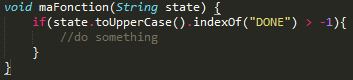
\includegraphics[scale=1]{Image/Extraction_Variable.png}\\
\itshape{Avant extraction de variable}
\end{center}

\paragraph{Exemple :}
Ci-dessus, nous pouvons voir une fonction qui va faire un traitement si l'état est "DONE".
Si l'on applique l'extraction de variable, on obtient une variable isDone qui contient un boolean. Cette méthode nous permet de passer d'un code qui contient une expression peu lisible à un code avec une variable explicite.

\begin{center}
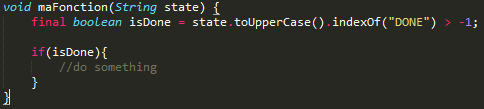
\includegraphics[scale=1]{Image/Extraction_Variable2.png}\\
\itshape{Après extraction de variable}
\end{center}

\paragraph{Bénéfices :}
Pour que le résultat de cette méthode soit optimal, il faut nommer efficacement les variables créées pour  qu'elles soient le plus lisible possible. Cela va permettre de produire un code plus lisible et qui contiendra moins de longs commentaires pour expliquer les longues expressions.

\paragraph{Inconvénient :}
Le code va contenir beaucoup de variables mais cela est dérisoire comparé à la lisibilité du code qui est nettement améliorée.

\paragraph{Technique inverse :}
La technique Inline Temp va permettre de supprimer les variables superflues qui contiennent uniquement le résultat d'une opération simple qui va être utilisé une seule fois. Cette technique n'a pas de vrai bénéfice dans cet état, en revanche elle peut être couplée avec la technique suivante.\\

\subsection{Remplacement des temporaires avec des méthodes}
\paragraph{Présentation :}
Le remplacement des temporaires avec des méthodes va comme son nom l'indique, remplacer des variables temporaires par le résultat de méthode. On va extraire le code des variables temporaires avec la technique Inline method puis les placer dans des méthodes.

\begin{center}
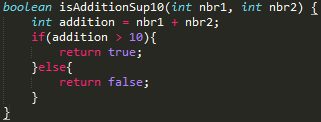
\includegraphics[scale=1]{Image/Remplacement_Temp_Methode.png}\\
\itshape{Avant remplacement du temporaire}
\end{center}

\paragraph{Exemple :}
Ci-dessus, nous pouvons voir que l'addition des deux paramètres est stockée dans une variable temporaire. Après le refactoring, la variable temporaire disparait et on obtient une méthode qui va s'occuper de faire l'addition à la place.

\begin{center}
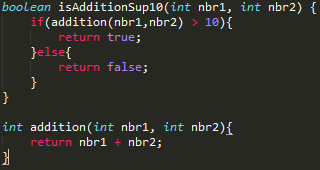
\includegraphics[scale=1]{Image/Remplacement_Temp_Methode2.png}\\
\itshape{Après remplacement du temporaire}
\end{center}

\paragraph{Bénéfices :}
Le code est plus compréhensible grâce au nom de la méthode qui est explicite.\\
Si j'ai besoin plus tard dans mon code de faire une addition, j'ai une méthode que je peux réutiliser.\\

\newpage

\subsection{Diviser les variables temporaires}
\paragraph{Présentation :}
Parfois dans notre code, nous déclarons une variable temporaire où nous stockons un résultat quelconque. Puis plus tard, nous réutilisons cette même variable pour stocker un tout autre résultat n'ayant aucun rapport.
Cette technique a pour but de ne plus utiliser la même variable temporaire pour faire différentes choses et de nommer proprement chaque variable temporaire.

\begin{center}
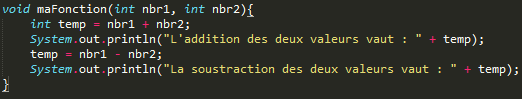
\includegraphics[scale=1]{Image/Diviser_Temp.png}\\
\itshape{Avant division}
\end{center}

\paragraph{Exemple :}
On peut voir au dessus que je réutilise la variable temp pour faire à la fois une addition et une soustraction. Après le refactoring on obtient deux variables proprement nommées addition et soustraction.

\begin{center}
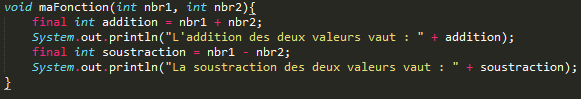
\includegraphics[scale=1]{Image/Diviser_Temp2.png}\\
\itshape{Après division}
\end{center}

\paragraph{Bénéfices :}
Le fait d'avoir chaque variable, méthode ou n'importe quel composant qui a un unique but ou une responsabilité, permet de faciliter grandement la maintenance du code, puisqu'on peut modifier des parties du code sans que ça affecte une autre partie.\\
Cela permet aussi une meilleure relecture du code car on supprime les variables nommées "tmp" ou "value" pour donner des noms facilement compréhensibles.\\

\subsection{Supprimer les assignations aux paramètres}
\paragraph{Présentation :}
Ici le problème est semblable à celui de la division des variables temporaires: si on a un paramètre, on ne doit pas lui affecter d'autre valeur car cela modifie ce que représente le paramètre et on peut se perdre dans le code car on ne sait plus ce que contient ce paramètre.\\
Il vaut donc mieux déclarer une variable locale plutôt que de modifier le paramètre.

\paragraph{Bénéfices :}
Comme dit plus haut, chaque élément a une unique responsabilité et la maintenance du code est plus simple.\\

\subsection{Remplacement de méthode par des objets}
\paragraph{Présentation :}
Il nous arrive d'écrire des méthodes très longues qui possèdent beaucoup de variables qui sont extrêmement liées entre elles. On peut avec le refactoring créer une nouvelle classe qui va contenir la méthode ainsi que les anciennes variables locales en variable de classe.

\begin{center}
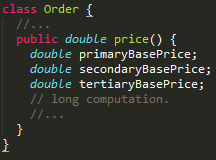
\includegraphics[scale=1]{Image/MethodeToObjet.png}\\
\itshape{Avant remplacement par l'objet \cite{ref5}}
\end{center}

\begin{center}
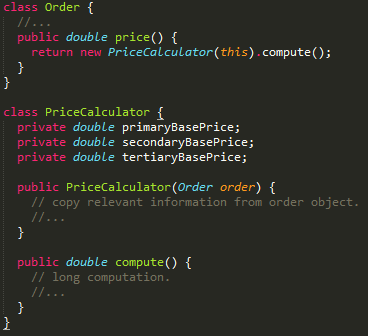
\includegraphics[scale=1]{Image/MethodeToObjet2.png}\\
\itshape{Après remplacement par l'objet \cite{ref5}}
\end{center}

\paragraph{Bénéfices :}
L'isolation d'une méthode longue dans sa propre classe permet d'empêcher le fait qu'elle ne prenne trop d'ampleur.\\
On peut aussi scinder cette méthode en sous-méthodes sans "polluer" la classe d'origine avec des méthodes utilitaires.

\paragraph{Inconvénient :}
Cette méthode de refactoring nous fait créer une nouvelle classe et cela augmente la complexité globale du programme.\\

\newpage

\section{Déplacement des fonctionnalités entre les objets}
Lorsque l'on code beaucoup de fonctionnalités dans un même programme, il arrive qu'au bout d'un moment, on se rende compte que , par exemple, on a placé une fonctionnalité dans la mauvaise classe. Et qu'on ne sait plus comment faire pour la déplacer sans risquer de casser tout le code.\\
Or les méthodes de refactoring qui vont suivre seront du type à permettre le déplacement de fonctionnalités entre des classes en toute sécurité.\\


\subsection{Déplacement de méthode}
\paragraph{Présentation :}
Il se peut qu'à un instant T, vous vouliez déplacer une méthode dans une autre classe car cela vous arrange ou car cela aurait plus de sens. Dans ce cas-là, on peut utiliser le refactoring pour déplacer cette méthode vers l'autre classe en toute sécurité.

\paragraph{Comment faire :}
Il faut commencer par regarder toutes les variables utilisées par la méthode et qui sont présentes dans la classe. Si ces variables ne sont utilisées que par la méthode à déplacer, il faut les déplacer dans la nouvelle classe aussi.\\
En revanche si ces variables sont utilisées par d'autres méthodes il est conseillé de déplacer aussi ces méthodes vers la nouvelle classe.
Ensuite, il faut s'assurer que toutes ces méthodes ne soient pas déclarées dans une classe mère ou fille.\\
Si toutes ces conditions sont réunies, on peut déclarer la ou les méthodes dans la nouvelle classe puis définir une méthode dans l'ancienne classe qui va appeler la nouvelle méthode.

\paragraph{Bénéfices :}
Cette méthode de refactoring nous permet d'obtenir une meilleure cohérence interne dans les classes.\\

\newpage

\subsection{Extraction de classe}
\paragraph{Présentation :}
Il est possible, lorsque l'on développe quelque chose, de créer une classe qui en réalité fait le travail de deux classes. Il vaut mieux modifier ça rapidement car cela risque d'empirer pour une classe illisible. On peut alors appliquer une technique de refactoring pour extraire une classe d'une autre.

\begin{center}
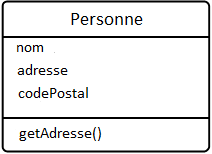
\includegraphics[scale=1]{Image/Extraction_Classe.png}\\
\itshape{Avant extraction de la classe}
\end{center}

\begin{center}
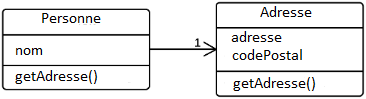
\includegraphics[scale=1]{Image/Extraction_Classe2.png}\\
\itshape{Après extraction de la classe}
\end{center}

\paragraph{Comment faire :}
Il faut d'abord créer la nouvelle classe ainsi qu'une relation entre l'ancienne et la nouvelle classe.\\
Ensuite, il faut utiliser les méthodes de refactoring "Déplacement de méthode" et "Déplacement de variable" pour toutes les variables et méthodes à déplacer.

\paragraph{Bénéfices :}
Cette méthode de refactoring permet de respecter le principe de responsabilité unique.
Les classes respectant ce principe sont plus fiables et tolérantes aux changements puisque si une classe peut faire plusieurs choses, la modification d'une fonctionnalité de la classe peut casser une autre fonctionnalité.

\paragraph{Technique inverse :}
La technique inverse consiste à supprimer les classes qui ont peu d'utilité. Cela permet de libérer de la mémoire.\\

\newpage

\subsection{Cacher la délégation}
\paragraph{Présentation :}
Nous sommes dans le cas où une structure permet à un client d'appeler une méthode d'un objet A qui lui renvoie un objet B pour ensuite appeler une méthode de l'objet B pour obtenir l'information souhaitée. On obtient une chaîne d'appels. Or si l'on veut changer quelque chose à la relation entre A et B, cela aura pour conséquence de changer la chaîne d'appels côté client.\\
Pour éviter ça, il est préférable de cacher la délégation au yeux du client à l'aide de refactoring.

\begin{center}
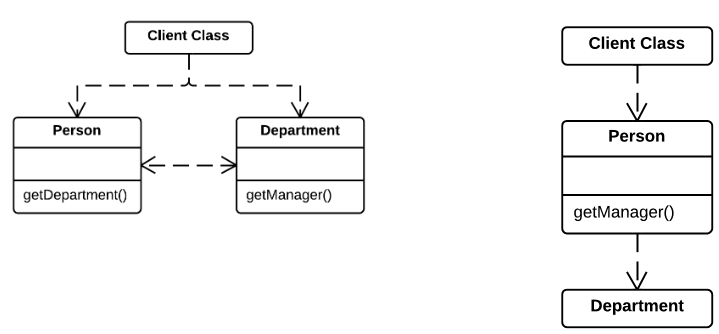
\includegraphics[scale=0.7]{Image/Cacher_Delegation.png}\\
\itshape{Avant/Après le refactoring \cite{ref5}}
\end{center}

\paragraph{Comment faire :}
Il faut commencer par créer dans la classe serveur (la classe dont le client a un access direct) les mêmes méthodes qui sont dans la classe déléguer (la classe qui contient les informations dont le client a besoin).\\
Ensuite, il faut changer le code client pour qu'il appelle la méthode de la classe serveur.\\
Si cela permet au client de ne plus avoir à utiliser la classe déléguer, on peut supprimer la méthode de la classe serveur qui renvoyait la classe déléguer.

\paragraph{Bénéfices :}
Le fait de cacher la délégation au client permet de lui cacher les relations entre les classes ce qui nous permet de changer le code de nos programmes plus simplement.

\paragraph{Inconvénient :}
A chaque fois qu'une nouvelle fonctionnalité est ajoutée à la classe déléguée, il faut créer une nouvelle méthode dans la classe serveur. Si ces changements arrivent souvent cela peut rapidement devenir pénible.

\paragraph{Technique inverse :}
Il existe donc une technique pour les cas où la classe déléguée possède beaucoup trop de méthodes : la technique de suppression du "Middle Man".
Cette technique consiste simplement à créer une méthode qui renvoie la classe déléguée pour éviter de devoir changer la classe serveur à chaque fois qu'une nouvelle fonctionnalité est ajoutée à la classe déléguée.\\


\newpage
\section{Organiser ses données}
Ce type de refactoring va permettre de mieux gérer les données des classes en dissociant les associations de classe pour les rendre plus portables et réutilisables.\\


\subsection{Auto Encapsulation des champs}
\paragraph{Présentation :}
Dans le cas d'une classe contenant des variables privées, il est préférable d'utiliser des getters et setters à l'intérieur même de la classe pour accéder aux variables.

\paragraph{Bénéfices :}
En accédant indirectement aux variables, on opte pour une approche plus flexible: cela nous permet par exemple de produire des opérations quand une variable est "set" ou "get". Cela peut être fait très facilement en modifiant simplement le getter et setter de la variable en question.
Utiliser les gettes et setters nous permet aussi de les redéfinir dans les sous-classes si un changement doit être fait dans les opérations de vérification.\\

\subsection{Passer du stockage par valeur en référence}
\paragraph{Présentation :}
Nous pouvons stocker des objets par valeur ou par référence. Le premier nous permet d'avoir une image de l'objet à l'instant où il est sauvegardé et le deuxième stocke un "lien" qui nous permet d'accéder à l'objet et non pas à une image.
Si lorsque nous créons un programme, nous stockons un objet qui ne change pas ou très peu dans le temps, nous pouvons le stocker par valeur; en revanche si à l'avenir cet objet vient à se modifier plus souvent, il sera nécessaire de le stocker par référence.

\paragraph{Bénéfices :}
Utiliser les références permet de posséder les informations les plus récentes à propos d'un objet. C'est à dire que si un objet est modifié à un moment, la personne qui possède une référence sur l'objet aura accès immédiatement au changement.

\paragraph{Inconvénient :}
L'inconvénient majeur de ce refactoring est qu'il est compliqué à mettre en place.

\paragraph{Technique inverse :}
Il est possible de faire le refactoring dans le sens inverse dans le cas où l'objet change très peu au fil du temps. Il ne vaut donc pas le coup de mettre en place une référence dans ce cas là.\\


\subsection{Remplacer les nombres magiques en constantes}
\paragraph{Présentation :}
Un nombre magique est un nombre qui n'est pas stocké dans une variable et qui apparait dans une équation, dont on ne connait pas l'utilité au premier coup d'œil. Il est très compliqué de modifier ces nombres magiques surtout s'ils apparaissent plusieurs fois dans le code.

\paragraph{Comment faire :}
La solution pour faire disparaître les nombres magiques et rendre le code plus lisible est très simple. Il suffit de trouver toutes les occurrences de ces nombres magiques et de déclarer une constante qu'on utilisera à la place. Cette constante aura un nom adapté pour que l'on puisse comprendre rapidement ce qu'elle représente.

\paragraph{Bénéfices :}
Les constantes permettent de savoir facilement leurs utilités de part leurs noms.\\
Il est beaucoup plus simple de changer la valeur d'une constante plutôt que de chercher partout dans le code.\\

\subsection{Encapsulation de collection}
\paragraph{Présentation :}
Dans le cas de l'utilisation d'une collection, il faut avoir en tête qu'il ne s'agit pas d'une simple variable qui nécessite un getter et un setter. Il faut la gérer différemment et créer des méthodes spécifiques pour la gestion de collection.

\paragraph{Comment faire :}
Pour traiter avec des collections, il faut un minimum de trois méthodes, la première étant la méthode "add". Cette méthode va permettre l'ajout d'un objet dans la collection en prenant uniquement l'objet à ajouter en paramètre.\\
La deuxième méthode est "remove", elle permet de supprimer un objet d'une collection en ne donnant que l'objet à effacer de la collection en paramètre.\\
La dernière est une simple méthode "get" qui va donner une copie de la collection pour que l'objet puisse être consulté sans pour autant pouvoir être modifié.

\paragraph{Bénéfices :}
Avec cette gestion de collection, on ne peut plus modifier une collection en récupérant l'objet à partir du getter.\\
Les règles, s'il y en a, pour ajouter des objets dans la collection seront toujours respectées puisqu'il faudra impérativement passer par la méthode add ou remove pour modifier la collection.\\
Cela permet aussi de rendre l'utilisation de collection plus simple.\\

\newpage

\subsection{Remplacer les Type Code}
\paragraph{Présentation :}
Les Type Code sont des champs qui peuvent contenir des valeurs fixes définis par le développeur pour représenter quelque chose.\\
Dans l'exemple ci-dessous, on a une classe qui représente une tâche à faire, et elle contient une variable qui va représenter son état qui peut être soit "TODO","ONGOING" ou "DONE". Ces trois états sont définis chacun par une valeur numérique.\\
Il existe trois types de refactoring qui permettent chacun de remplacer les Type Code par des alternatives plus avantageuses.

\begin{center}
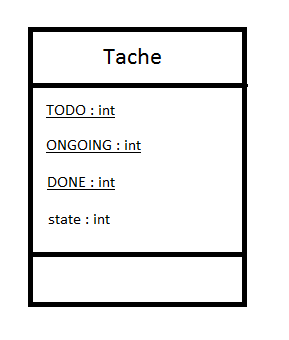
\includegraphics[scale=1]{Image/TypeCode.png}\\
\itshape{Exemple de Type Code}
\end{center}

\paragraph{Remplacement par une classe :}
Il est possible de remplacer un Type Code par une classe de type Énumération.\\
Cela permet de ne plus utiliser de simples nombres qui ne sont pas forcément compréhensibles à première vue alors que les énumérations sont facilement lisibles.\\
Le typage à l'aide d'une énumération va permettre de ne plus se soucier de la valeur des Type Code (Est ce que le nombre rentré a bien une signification?) ce qui permet de faire moins de gestion sur ces valeurs.

\begin{center}
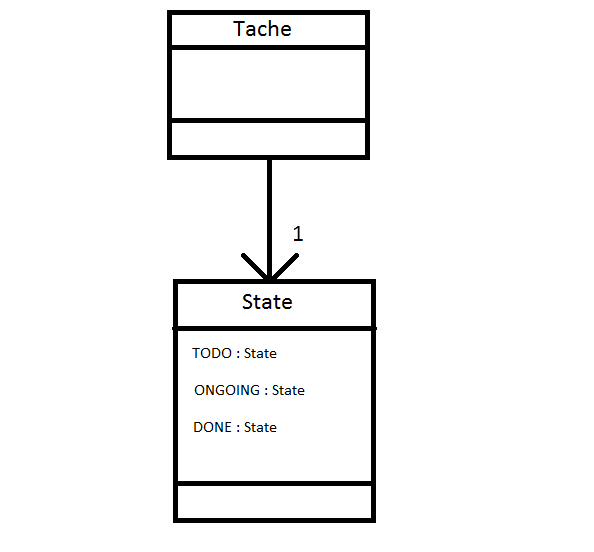
\includegraphics[scale=1]{Image/TypeCodeClasse.png}\\
\itshape{Remplacement de Type Code à l'aide d'une classe}
\end{center}

\paragraph{Remplacement par une sous classe :}
On peut remplacer les Type Code par des sous-classes. A l'aide de ce procédé nous pouvons écrire des méthodes ou créer des champs spécifiques selon le type de l'objet. Cette méthode permet aussi de rajouter très facilement de nouveaux "types" en créant simplement une nouvelle sous-classe.
Elle adhère aussi mieux au principe de responsabilité unique.\\
En revanche, le problème de cette approche est qu'on ne peut pas modifier le type de l'objet facilement s'il venait à changer.\\
Il est possible de faire la technique inverse dans le cas où les sous-classes diffèrent uniquement par les valeurs retour des méthodes (ces valeurs étant des constantes). Garder des sous classes dans ce cas là complexifie l'architecture pour un apport négligeable.

\begin{center}
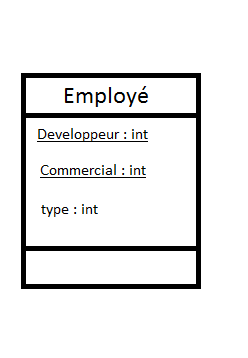
\includegraphics[scale=1]{Image/TypeCode_SousClasse.png}\\
\itshape{Avant remplacement de Type Code à l'aide d'une sous classe}
\end{center}

\begin{center}
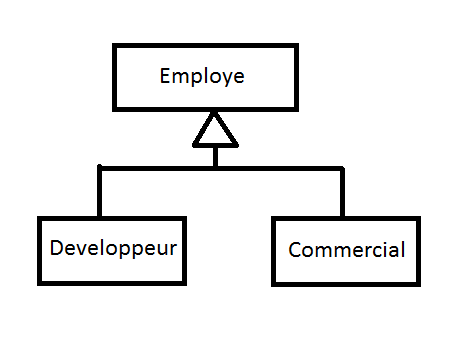
\includegraphics[scale=1]{Image/TypeCode_SousClasse2.png}\\
\itshape{Après remplacement de Type Code à l'aide d'une sous classe}
\end{center}

\paragraph{Remplacement par State/Strategy}
Cette méthode est une alternative à la précédente dans le cas où le type de l'objet est soumis à des changements pendant sa durée de vie. Cette méthode utilise le pattern State/Strategy. Comme la précédente, il est simple de rajouter une nouveau type si besoin sans avoir à modifier du code existant. L'exemple suivant est le même que le précédent.

\begin{center}
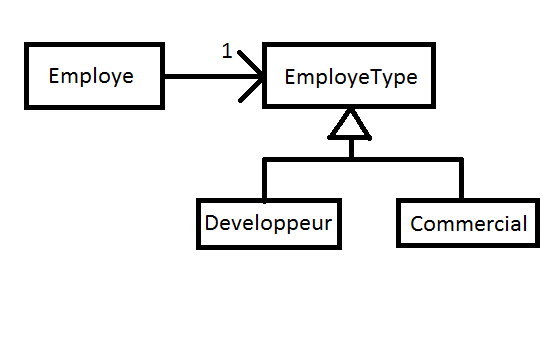
\includegraphics[scale=1]{Image/TypeCode_State.png}\\
\itshape{Après remplacement de Type Code à l'aide du pattern State/Strategy}
\end{center}


\newpage
\section{Simplifier les expressions conditionnelles}
Dans les programmes, il n'est pas rare de trouver des expressions conditionnelles qui possèdent une logique complexe avec beaucoup de conditions. Ce type de refactoring va permettre de simplifier toutes ces expressions.\\



\subsection{Décomposer les expressions conditionnelles}
\paragraph{Présentation :}
Il nous arrive souvent, dans nos programmes, d'avoir des conditions regroupant plusieurs conditions. Le résultat étant une condition assez complexe à comprendre sans commentaire pour l'expliquer. La solution à ce problème est de déplacer le calcul de ces conditions dans des méthodes.

\paragraph{Comment faire :}
Pour ce faire, il faut utiliser la méthode de refactoring d'extraction de méthode sur le bloc conditionnel pour obtenir un simple appel de méthode avec un nom compréhensible.

\paragraph{Bénéfices :}
Le bénéfice majeur de cette technique est de permettre une relecture et une maintenance du code simplifiées.\\

\subsection{Remplacer les conditions avec du polymorphisme}
\paragraph{Présentation :}
Dans le cas où nous avons par exemple un switch qui va produire différents traitements selon le type d'un objet, il sera intéressant de supprimer le switch pour produire des sous classes.

\begin{center}
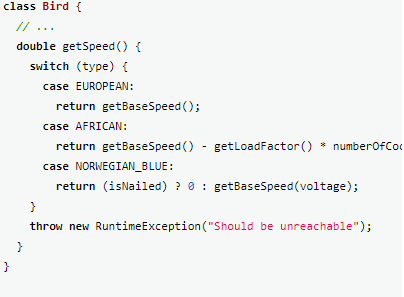
\includegraphics[scale=1]{Image/ReplaceConditionalPoly.png}\\
\itshape{Avant refactoring \cite{ref5}}
\end{center}

\paragraph{Exemple :}
Dans l'exemple, on est passé d'un switch qui calculait la vitesse d'un oiseau selon son type dans la classe "Bird" à une classe abstraite qui nécessite la redéfinition de la méthode de calcul de vitesse afin que chaque sous-classe soit obligée de la redéfinir.

\begin{center}
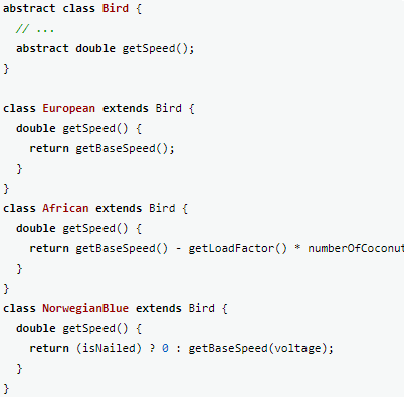
\includegraphics[scale=1]{Image/ReplaceConditionalPoly2.png}\\
\itshape{Après refactoring \cite{ref5}}
\end{center}

\paragraph{Bénéfices :}
Dans cet exemple cela permettrait de rajouter des types d'oiseaux simplement en recréant une sous classe sans avoir à modifier une méthode déjà existante.\\
On évite aussi des conditions switch ou autres très longues du fait qu'il y aurait beaucoup de types à gérer.\\

\newpage

\subsection{Introduire des assertions}
\paragraph{Présentation :}
Une assertion est une expression qui doit être évaluée à vrai pour que le programme puisse continuer à fonctionner. Si une assertion est évaluée faux alors le programme s'arrête immédiatement.
Dans le cadre d'un programme qui nécessite absolument une variable, un objet ou n'importe quoi pour pouvoir fonctionner, même si cette donnée est censée être présente à ce moment du programme, il est plus sûr de placer une assertion pour vérifier que cette donnée existe bien au moment venu.

\paragraph{Bénéfices :}
Placer des assertions permet de détecter des erreurs et permet d'arrêter des programmes qui risquent de faire des dégâts si on les laisse continuer alors que quelque chose ne s'est pas déroulé comme prévu.
Les assertions sont la plupart du temps utilisées dans les tests unitaires mais elles peuvent être utilisées dans nos programmes et se révéler très utiles.\\

\newpage
\section{Simplifier les appels de méthode}
Ces techniques de refactoring ont pour but de simplifier l'appel de méthode et rendre l'appel de méthode plus facile à comprendre.\\



\subsection{Renommer une méthode}
\paragraph{Présentation :}
Commençons cette partie par quelque chose de simple mais terriblement efficace, les noms de méthode.\\
Lorsque l'on code une méthode, il faut lui donner un nom qui permet de comprendre ce que la méthode fait sans avoir à lire une seule ligne de code. Il s'agit d'une règle de base en programmation mais elle n'est pas toujours respectée.

\paragraph{Bénéfices :}
L'avantage de bien nommer une méthode est d'améliorer la relecture de son propre code ainsi que grandement faciliter la future maintenance du code par quelqu'un d'autre.\\

\subsection{Séparer les requêtes de questionnement et de modification}
\paragraph{Présentation :}
Une méthode doit avoir une seule tâche à accomplir et non plusieurs, surtout si cette même méthode mêle opération de lecture et d'écriture.
Dans cette méthode de refactoring, nous appliquons le pattern de "Command and Query Responsibility Segregation" qui nous dit qu'il faut séparer les opérations de lecture et d'écriture.
Pour appliquer ce refactoring il faut simplement séparer la méthode en deux pour obtenir deux nouvelles méthodes, une qui récupère des données et l'autre qui modifie des données.

\paragraph{Bénéfices :}
Cette technique permet évidemment de pouvoir faire des lectures sans avoir forcement à modifier une donnée.\\
Le pattern "Command and Query Responsibility Segregation" nous permet de maximiser les performances, l'évolutivité ainsi que la sécurité.\\

\newpage

\subsection{Méthode paramétrée}
\paragraph{Présentation :}
Parfois, il peut nous arriver d'écrire deux méthodes assez similaires qui ont un but commun mais qui le traitent avec des opérations ou valeurs qui diffèrent. Dans un cas similaire, il est conseillé de créer une seule méthode qui va regrouper les deux et prendre un paramètre pour savoir quel traitement appliquer.\\

\begin{center}
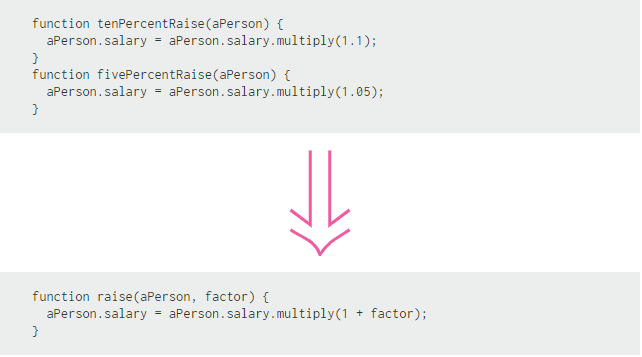
\includegraphics[scale=1]{Image/Methode_Parametre.png}\\
\itshape{Exemple de méthode paramétrée \cite{ref8}}
\end{center}

\paragraph{Bénéfices :}
On obtient une seule méthode au lieu de deux très similaires, ce qui permet la suppression de la duplication de code.\\
A l'avenir, on n'a plus besoin de créer d'autres méthodes si une nouvelle version de la méthode est nécessaire comme une augmentation de sept pour cent en reprenant l'exemple.\\

\paragraph{Technique inverse :}
Il existe une technique qui revient plus ou moins à faire l'inverse. Il s'agit de la méthode de remplacement de paramètres avec des méthodes explicites.\\
Dans ce cas, on a une méthode qui va pouvoir faire plusieurs traitements différents qui n'ont rien à avoir entre eux. La méthode sait quel traitement faire grâce à un des paramètres.\\
On peut avoir une méthode "setValue" qui prend en paramètre une chaîne de caractères et une valeur. Si la chaîne est "prix" alors la méthode sauvegarde la valeur dans le prix et si la chaîne est "poids" alors la méthode va enregistrer la valeur dans la variable poids.\\
Il serait donc préférable de faire du refactoring et de séparer les deux méthodes pour obtenir une méthode "setPrix" et une autre "setPoids". Ce qui rend le programme plus clair et intuitif.\\

\subsection{Conserver l'objet entier}
\paragraph{Présentation :}
Lorsqu'une méthode a besoin de variables qui sont contenues dans un objet, il est préférable d'envoyer l'objet entier en paramètre plutôt que d'envoyer uniquement les variables de l'objet.

\paragraph{Bénéfices :}
Le résultat est un code plus lisible car on n'a plus qu'un paramètre qui est l'objet contenant tous les anciens paramètres.\\
Un autre avantage : si la méthode doit évoluer et a besoin d'une autre variable de l'objet, pas besoin d'aller modifier tout le code pour modifier l'appel de la méthode en rajoutant le nouveau paramètre. Cela rend le code plus facile à faire évoluer.\\

\subsection{Ajouter des objets en paramètre}
\paragraph{Présentation :}
Dans nos programmes, il peut arriver que l'on écrive plusieurs méthodes utilisant exactement les mêmes paramètres. Le problème étant une duplication de paramètres ainsi que potentiellement une duplication de code à l'intérieur des méthodes en traitant les paramètres.\\
Dans ce cas, nous avons la possibilité de créer un objet qui va contenir les paramètres ainsi que des méthodes qui vont s'occuper du traitement de ces paramètres.\\

\begin{center}
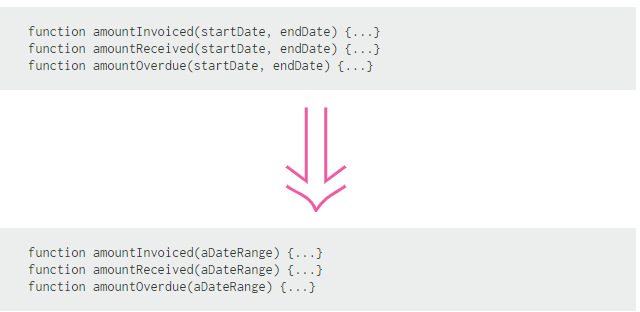
\includegraphics[scale=1]{Image/Ajout_Objet_Parametre.png}\\
\itshape{Exemple de transformation de paramètre en objet \cite{ref8}}
\end{center}

\paragraph{Bénéfices :}
L'avantage principal de cette méthode est de supprimer la duplication de code générée par le traitement identique des paramètres dans plusieurs méthodes.\\
Les paramètres sont aussi plus lisibles du fait qu'il ne reste plus qu'un seul objet avec un nom adapté pour une compréhension simple et efficace.\\
En revanche, ce refactoring est inutile s'il sert uniquement à stocker les paramètres sans y ajouter des méthodes de traitement.\\

\subsection{Remplacer les constructeurs par des méthodes Factory}
\paragraph{Présentation :}
Plaçons-nous dans un cas où on veut que notre constructeur ne soit pas accessible par l'extérieur.
On va alors devoir utiliser cette méthode de refactoring qui se base sur le pattern de factory.

\paragraph{Comment faire :}
Pour ce faire, il faut simplement créer une nouvelle méthode avec un nom adapté comme "createNomObjet", cette méthode va alors appeler elle-même le constructeur et renvoyer une instance de l'objet demandé.

\paragraph{Bénéfices :}
Les méthodes de type Factory ne renvoient pas forcément une instance de l'objet dont elles font partie. Cela peut avoir un grand avantage s'il faut renvoyer une sous-classe car on peut utiliser cette méthode pour faire un traitement à l'aide de paramètres pour décider quelle sous-classe renvoyer.\\
La méthode Factory peut avoir un nom plus approprié que celui d'un constructeur afin de comprendre ce qu'elle fait.\\
On peut aussi l'utiliser pour renvoyer des instances déjà existantes(Singleton), ce qui n'est pas possible avec un constructeur.\\

\newpage

\subsection{Remplacer les codes d'erreurs par des exceptions}
\paragraph{Présentation :}
Aujourd'hui il vaut mieux éviter d'utiliser les codes d'erreurs car il existe une classe spécialement faite pour la gestion d'erreurs, les exceptions.\\
L'utilisation des exceptions permet de détecter et de traiter les erreurs qui peuvent se produire pendant l'exécution du code.\\

\begin{center}
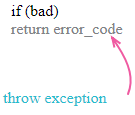
\includegraphics[scale=1]{Image/ThrowException.png}\\
\itshape{Remplacement de code d'erreur par une exception \cite{ref8}}
\end{center}

\paragraph{Bénéfices :}
L'utilisation des exceptions nous permet principalement d'éviter de faire de la gestion d'erreur à travers les codes d'erreurs.\\
Il est plus rapide de se rendre compte que quelque chose s'est mal passé si une exception est levée.\\
Les codes d'erreurs ne peuvent pas être utilisés dans les constructeurs alors que les exceptions le peuvent.\\
On peut aussi créer nos propres exceptions pour qu'elles fassent un traitement particulier.\\

\paragraph{Méthode alternative :}
Les exceptions sont des objets qui doivent être utilisés pour gérer les comportements irréguliers provoqués par des erreurs inattendues.\\
Il ne faut pas utiliser les exceptions à la place de simple test.\\

\begin{center}
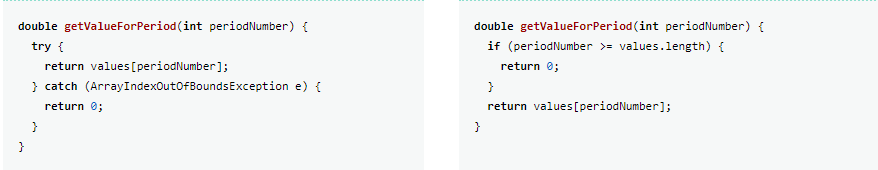
\includegraphics[scale=0.75]{Image/ExceptionTest.png}\\
\itshape{Remplacement d'exception par un test \cite{ref5}}
\end{center}

\newpage
\section{Faire face à la généralisation}
Dans cette partie, nous allons étudier des techniques permettant de déplacer des fonctionnalités dans la hiérarchie d'héritage de classes, à la création de nouvelles classes et d'interfaces.\\



\subsection{Remonter les variables et méthodes}
\paragraph{Présentation :}
Nous allons commencer par un cas basique : si nous avons une super classe ainsi que deux sous-classes qui héritent de la super classe, et que les deux sous-classes possèdent un attribut ou une méthode commune que ne possède pas la super classe alors il sera intéressant de déplacer cette variable ou méthode dans la super classe.\\

\paragraph{Bénéfices :}
Ce refactoring élimine de la duplication de code que ce soit dans la définition d'une variable ou méthode ou bien pour le corps de la méthode.\\
Dans le cas de la méthode cela permet de ne modifier que la méthode présente dans la super classe en cas de changement au lieu de devoir passer dans toutes les sous-classes.\\

\paragraph{Technique inverse :}
Il existe évidemment une technique pour descendre les champs et méthodes.\\
Que ce soit pour les variables ou les méthodes, il est préférable de déplacer un champ ou une méthode d'une super classe dans une sous-classe si ce dit champ ou méthode n'est utilisé que dans cette même sous-classe.\\
Cela permet de rendre le code plus compréhensible et améliore la cohérence interne de la classe.\\


\subsection{Extraire une super classe}
\paragraph{Présentation :}
Si l'on a deux classes qui possèdent des champs ou des méthodes communs, alors il serait intéressant de créer une super classe dont les deux classes hériteraient.\\

\paragraph{Bénéfices :}
On supprime donc de la duplication de code.\\
En revanche cette méthode de refactoring ne peut pas être utilisée dans le cas où l'une des deux classes possèdent déjà une super classe.\\

\subsection{Créer des méthodes Template}
\paragraph{Présentation :}
Il nous est déjà arrivé d'avoir deux sous-classes qui possèdent une méthode assez similaire qui déroule un algorithme possédant les mêmes étapes mais avec des valeurs changeantes.\\
Il y a alors un moyen de créer un template de la méthode dans la super classe tout en laissant l'implémentation qui diffère aux sous-classes.\\

\begin{center}
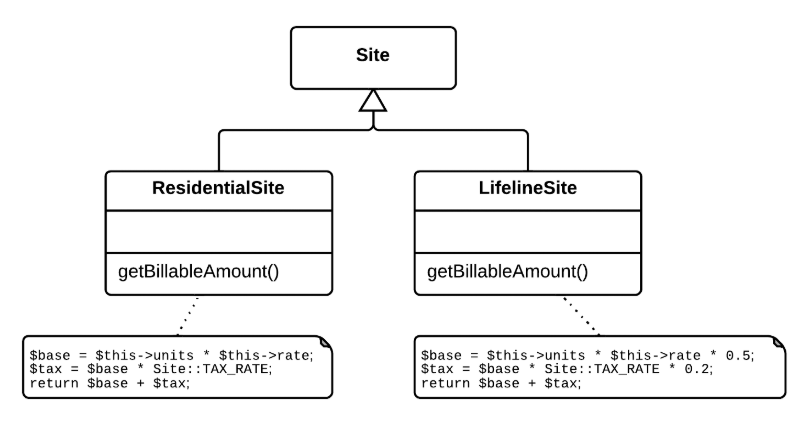
\includegraphics[scale=0.75]{Image/Template.png}\\
\itshape{Avant mise en place du template \cite{ref5}}
\end{center}

\paragraph{Exemple :}
Dans l'exemple ci-dessus, on peut voir qu'on a deux sous-classes qui possèdent une méthode permettant de calculer le montant d'une facture.\\
Les deux méthodes n'utilisent pas les mêmes valeurs pour le calcul mais en revanche le calcul se résume dans les deux cas à l'addition du tarif de base additionné aux taxes.\\
On peut donc voir ci-dessous que la solution est de remonter la méthode de calcul du montant de la facture dans la super classe. Celle-ci va renvoyer l'addition du prix de base additionné à celui des taxes.\\
Ces prix-là seront calculés à l'aide de deux nouvelles méthodes qui seront redéfinies dans les sous-classes.\\

\begin{center}
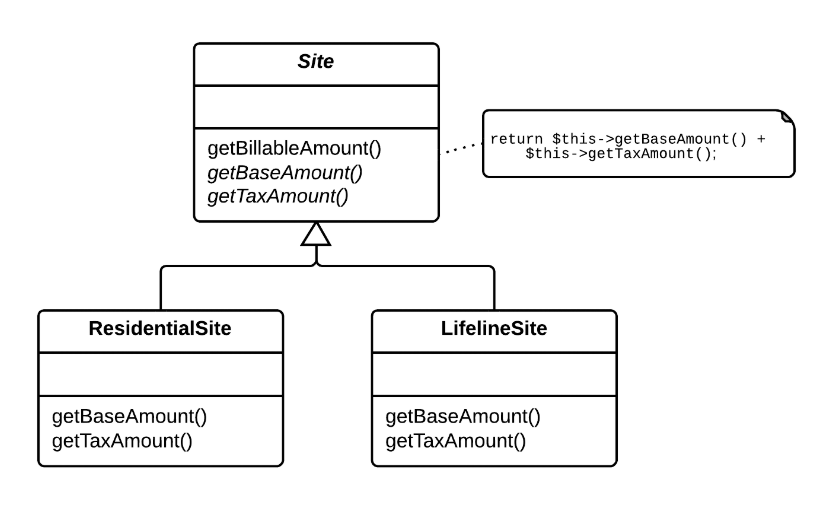
\includegraphics[scale=0.75]{Image/Template2.png}\\
\itshape{Après mise en place du template \cite{ref5}}
\end{center}

\paragraph{Bénéfices :}
Les templates nous permettent de supprimer de la duplication de code même s'il ne s'agit pas exactement du même code.\\
Cela peut aussi nous faire gagner du temps dans le cas où il faut créer une nouvelle sous-classe. Dans l'exemple il suffira de redéfinir le calcul du prix de base et des taxes.\\

\newpage

\subsection{Remplacer l'héritage par de la délégation}
\paragraph{Présentation :}
Ici, nous avons une classe B qui hérite d'une classe A et qui n'utilise qu'une petite portion des méthodes de sa super classe.\\
Il serait judicieux de créer un champ dans B pour stocker A et ensuite de créer des méthodes pour déléguer le travail à la classe A.\\

\paragraph{Bénéfices :}
Cela permet à la classe B de posséder uniquement les méthodes qu'elle utilise et non pas toutes les méthodes de la classe A qu'elle n'utilise pas.\\

\paragraph{Technique inverse :}
Il existe aussi la technique inverse, c'est à dire remplacer la délégation par de l'héritage dans le cas où la classe B utilise beaucoup de méthodes de la classe A.
Dans ce cas il est préférable de privilégier l'héritage afin de réduire la taille du code due à la suppression de toutes les méthodes de délégation.\\

\chapter{Les graphes de flots de contrôle dans le refactoring}

\section{Présentation}

\subsection{Définition}
Un graphe de flot de contrôle est une représentation sous forme de graphe de tous les chemins qui peuvent être suivis par un programme durant son exécution.\\
Il s'agit de graphe orienté.\\
Voici comment sont représentés les différents types d'instructions dans les graphes de flots de contrôle.\\
Les exemples ci-dessous sont tirés du site "geeksfirgeeks.org" \cite{ref18}\\

Instruction If-Else :

\begin{center}
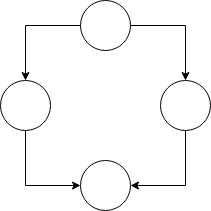
\includegraphics[scale=1]{Image/ExempleIfElse.png}\\
\itshape{Exemple de bloc If Else dans un graphe de flots de contrôle}
\end{center}

\newpage

Instruction While :

\begin{center}
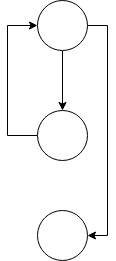
\includegraphics[scale=1]{Image/ExempleWhile.png}\\
\itshape{Exemple de bloc while dans un graphe de flots de contrôle}
\end{center}

Instruction Do While : 

\begin{center}
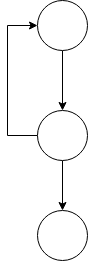
\includegraphics[scale=1]{Image/ExempleDoWhile.png}\\
\itshape{Exemple de bloc do while dans un graphe de flots de contrôle}
\end{center}

\newpage

Chaque graphe de flots de contrôle possède un sommet entrée (là où le programme débute) et un sommet sortie (là où le programme termine).\\
Les autres sommets représentent des blocs d'instructions et les arcs la possibilité de transfert de l'exécution d'un nœud à un autre \cite{ref11}.

\begin{center}
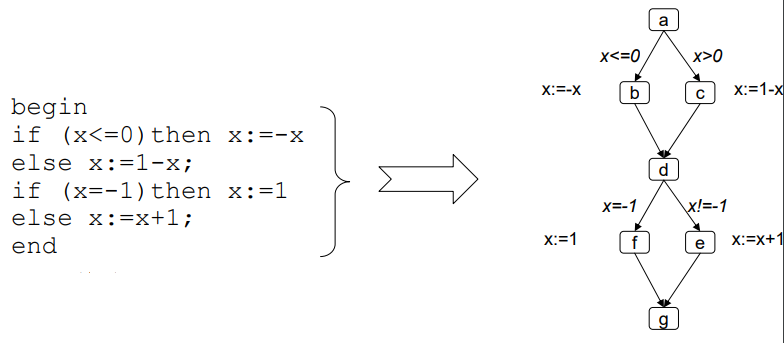
\includegraphics[scale=0.7]{Image/GFC.png}\\
\itshape{Exemple de graphe de flots de contrôle\cite{ref11}}
\end{center}

Une exécution possible est représentée par un chemin de contrôle dans le graphe de contrôle. Un chemin de contrôle doit impérativement commencer par le sommet entrée et finir par le sommet sortie.\\
Un exemple de chemin de contrôle : [a,c,d,e,g].\\
Il est possible de représenter sous forme algébrique l'ensemble des chemins de contrôle du graphe (M).\\
Ici on aurait :\\
M = a.(b+c).d.(e+f).g\\

Les blocs présents dans les graphes de flots de contrôle possèdent des relations de domination entre eux.\\
On peut dire "qu'un bloc M domine un bloc N si chaque chemin qui atteint le bloc N passe par M"\cite{ref17}.\\
Cette définition montre que le bloc entrée domine n'importe quel bloc puisque tout chemin débute par le bloc entrée.\\
On peut aussi dire que M postdomine N si "chaque chemin de N vers le bloc de sortie passe par M"\cite{ref17}\\
On parle aussi de domination immédiate dans le cas où un bloc M est le dernier dominant de N en partant du bloc entrée. Un bloc ne peut donc être dominé immédiatement par un seul bloc.\\
On peut analyser toutes ces relations de domination entre les blocs en générant un arbre de dominance.\\
Voici un exemple d'arbre de dominance par rapport à l'exemple de graphe de flots de contrôle situé plus haut.

\begin{center}
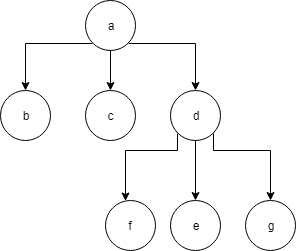
\includegraphics[scale=1]{Image/ArbreDominance.png}\\
\itshape{Exemple d'arbre de dominance}
\end{center}

On a donc f,e,g qui sont dominés par a et d.\\
Et b,c,d qui sont dominés par a.\\


\subsection{Sont-ils utilisables pour faire du refactoring ?}
Actuellement il n'existe pas de logiciel utilisant les graphes de flots de contrôle pour effectuer du refactoring.\\
Théoriquement il n'est pas impossible de faire du refactoring avec ce type de graphe.
D'après un article de recherche traitant du test structurel des exécutables, il est possible à l'aide des flots de contrôle de détécter si tous les noeuds ou tous les arcs peuvent être atteints\cite{ref12}.\\
Dans un autre article on nous dit qu'en utilisant les graphes de flots de contrôle couplés à l'exécution symbolique, il est possible de détecter des chemins infaisables\cite{ref20}.\\
Cet aspect pourrait être utilisé dans le refactoring pour détecter du code non accessible lors de l'exécution du programme.\\
On pourrait aussi utiliser une détection de chemin
permettant une optimisation du code en empruntant un chemin moins coûteux en temps et ressources.\\
En revanche, on ne peut pas utiliser les graphes de flots de contrôle pour tester tous les chemins possibles d'un programme dès lors qu'il contient des boucles car le nombre de chemins va être infini.\\

\newpage

\section{Détection du code mort avec les graphes de flots de contrôle}

\subsection{L'exécution symbolique}
Je vais maintenant vous parler de l’exécution symbolique, technique d’analyse de programmes nécessaire pour la partie du refactoring avec les graphes de flots de contrôle.\\
L’exécution symbolique ne doit pas être confondue avec l’exécution concrète.\\
Pour simplifier ce point, je vais vous présenter un exemple.\\

\begin{center}
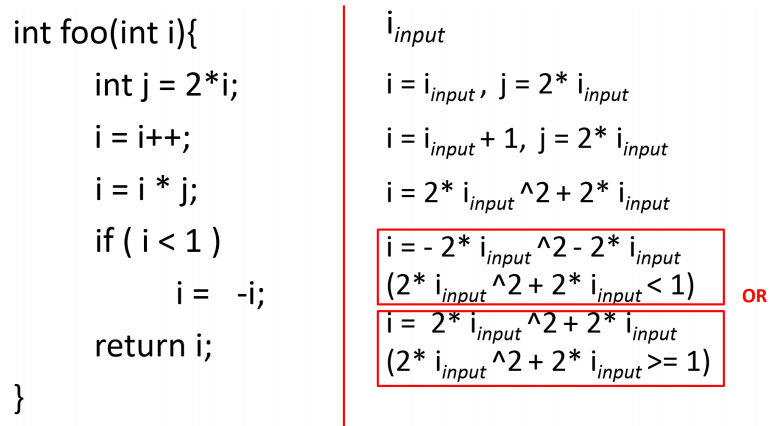
\includegraphics[scale=0.8]{Image/ExempleExecutionSymbolique.png}\\
\itshape{Exemple d'exécution symbolique \cite{ref15}}
\end{center}

A gauche, nous avons l’exécution concrète et à droite l’exécution symbolique.\\
On peut voir que lors de l’exécution symbolique, on s’intéresse exclusivement aux valeurs des différentes variables présentes dans le programme.\\
Ces valeurs ne sont pas définies avec des valeurs réelles mais avec des inconnues; la valeur de i et j dépend principalement du paramètre i appelé i input.\\
L’exécution symbolique a plusieurs applications.
On peut par exemple générer des tests sur les inputs, trouver des bugs et des vulnérabilités dans les programmes.\\
Mais ici l’utilisation qui nous intéresse est la détection de chemin infaisable.\cite{ref15}\\
D’après James C. King, il faut que les variables utilisées dans les programmes soient uniquement des nombres entiers pour pouvoir effectuer l’exécution symbolique.\cite{ref16}

\subsection{Arbre d'exécution symbolique}

Les arbres d’exécution symbolique sont des représentations de l’exécution symbolique.\\

D’après James C. King, les arbres d’exécution symbolique sont, pour la plupart des programmes, infinis.\cite{ref16}\\
Cela pourrait être un point bloquant si on veut utiliser cette solution couplée aux graphes de flots de contrôle pour faire du refactoring. Il faudrait se limiter à des programmes avec lesquels on peut générer un arbre d'exécution symbolique fini.\\
On va directement étudier un exemple pour mieux comprendre de quoi est formé un arbre d’exécution symbolique.\\

\begin{center}
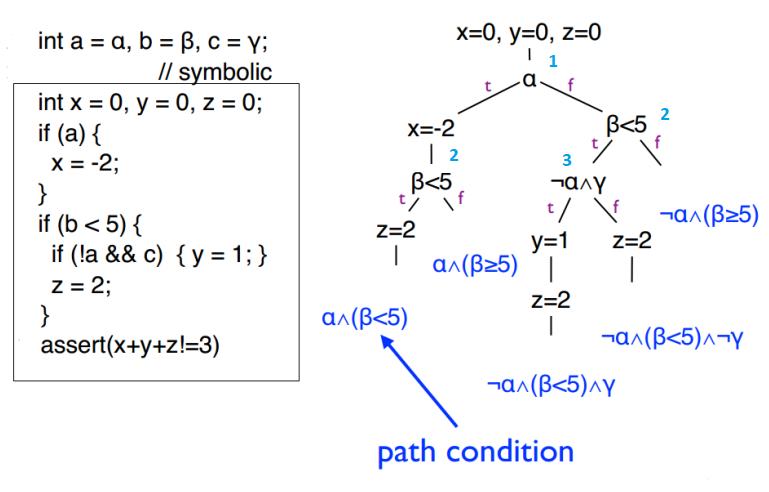
\includegraphics[scale=0.8]{Image/ExempleArbreExecutionSymbolique.png}\\
\itshape{Exemple d'un arbre d'exécution symbolique \cite{ref15}}
\end{center}

Sur l’exemple on a l’exécution symbolique qui nous dit que la variable a vaut alpha, b vaut beta et c vaut gamma.\\

Le point 1 (alpha) sur l’arbre d’exécution symbolique représente la condition " if (a) ": elle signifie que si alpha est évalué à true, on prend la branche de gauche. Sinon on prend la branche de droite.\\

Le point 2 (beta < 5) représente la condition " if (b<5) ": si l’on prend le chemin de gauche c’est que l’évaluation de la condition est vraie et donc fausse pour le chemin de droite.\\

Le point 3 (not alpha et gamma) représente la condition " if (!a ET c) " et comme pour les précédents, le chemin de gauche est l’évaluation à true et false pour le chemin de droite.\\

Au niveau des feuilles de l’arbre, on peut voir en bleu des conditions de chemin.\\
Il s’agit des conditions nécessaires à remplir pour pouvoir atteindre cet endroit de l’arbre d’exécution symbolique.\\

Par exemple si l’on a : (alpha ET (beta < 5)) cela veut dire que pour accéder à cette branche, il faut que alpha soit évalué à true et que beta soit inférieur à 5.\\
Et c’est à l’aide de ces conditions de chemin que l’on va pouvoir déterminer quels sont les chemins qui ne peuvent pas être atteints.\\

\subsection{Le solveur Z3}

Dans le cas où on a pu générer un arbre d’exécution symbolique qui contient uniquement des variables de type Integer et qui n’est pas infini, on va pouvoir utiliser le solveur Z3. Le solveur Z3 est un démonstrateur automatique de théorème, c’est-à-dire qu’il peut résoudre n’importe quelle équation du moment qu’il existe au moins une solution.\\
Il s’agit d’un projet de Microsoft développé en C++. Ce solveur est applicable sur plusieurs langages de programmation dont le Java dans notre cas.\\
Le solveur Z3 va nous permettre de résoudre toutes les conditions de chemin pour savoir s’il est possible ou non d’accéder à ce chemin ou tout simplement détecter si les chemins sont faisables ou pas.\\
Il nous est donc possible de détecter des chemins infaisables à l'aide de l'exécution symbolique et du solveur Z3.\\


\newpage



\subsection{Exemple d'utilisation possible d'un graphe de flots de contrôle dans le refactoring}

Ci-dessous une manière d'utiliser les graphes de flot de contrôle dans le refactoring et plus précisément pour détecter du code mort.\\
A l'aide du test structurel qui utilise les graphes de flot de contrôle, il est possible d'avoir une couverture de toutes les décisions possibles\cite{ref13}.\\
C'est à dire de trouver au moins un ensemble de combinaisons de valeurs qui permet de passer toutes les conditions du programme. Cette technique pourrait donc être utilisée dans le refactoring pour détecter du code mort car dans le cas où il n'existe aucun ensemble de combinaisons de valeur permettant de satisfaire toutes les conditions, alors on peut trouver la partie du programme inatteignable (code mort).\\

\begin{center}
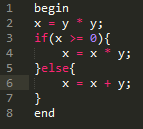
\includegraphics[scale=1.5]{Image/ExempleCodeGraphe.png}\\
\itshape{Code à analyser avec le graphe de flots de contrôle}
\end{center}

\begin{center}
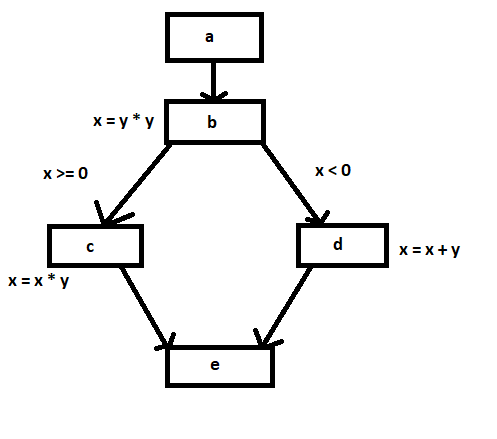
\includegraphics[scale=0.8]{Image/ExempleGraphe.png}\\
\itshape{Graphe de flots de contrôle généré à partir du code ci-dessus}
\end{center}

Imaginons que dans l'exemple une variable y soit générée aléatoirement entre -100 et 100.
L'exemple ci-dessus est très simple mais a pour but de montrer qu'il est possible de détecter du code mort.\\
On a donc une variable x à laquelle on affecte le carré d'une variable y, or le carré de n'importe quel entier est positif ou nul.\\ Si on regarde le mini programme, on peut facilement comprendre que jamais on ne pourra passer par le else car x ne peut pas être négatif. Mais imaginons que ce soit un programme beaucoup plus compliqué.\\
On va alors générer un arbre d’exécution symbolique à partir du code présenté ci-dessus.\\
Un algorithme qui permet de générer un arbre d'exécution symbolique a été proposé dans un article\cite{ref20}.\\
Et on obtiendra l’arbre ci-dessous.\\


\begin{center}
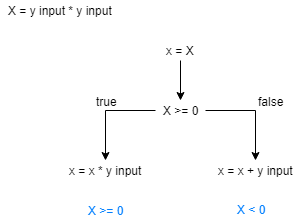
\includegraphics[scale=0.9]{Image/ExempleArbreExecutionSymbolique2.png}\\
\itshape{Arbre d'exécution symbolique généré}
\end{center}

Sur notre arbre d'exécution symbolique, on peut voir en bleu les conditions de chemins qui doivent être résolubles si l'on veut pouvoir affirmer qu'il s'agit d'un chemin faisable.\\
Pour ce faire il nous suffit d'utiliser le solveur Z3 pour nous aider à résoudre ces équations.\\
Le solveur va alors nous dire qu'il est possible de résoudre l'équation "X>=0" mais en revanche il nous dira qu'il est impossible de trouver une solution à l'équation "X<0".\\
Maintenant que l'on connait les chemins qui sont infaisables, il nous suffit de régénérer le graphe de flots de contrôle en coloriant en rouge les blocs inaccessibles et en vert les blocs accessibles.\\
On obtient donc un nouveau graphe de flot de contrôle facilement compréhensible pour visualiser où se trouve le code mort du programme.


\begin{center}
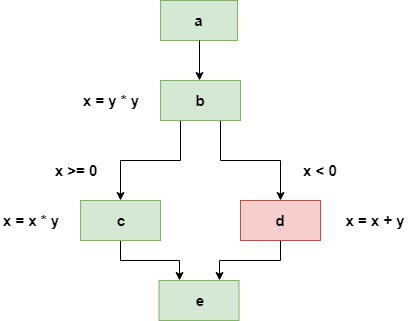
\includegraphics[scale=0.8]{Image/ExempleGraphe2.png}\\
\itshape{Graphe de flots de contrôle généré après analyse de l'arbre d'exécution symbolique}
\end{center}

Le graphe de flots de contrôle nous permettrait donc de détecter du code mort en étudiant les décisions possibles d'un programme à l'aide de l'exécution symbolique.\\
En revanche la complexité de l'algorithme qui détecte toutes les décisions possibles est exponentiel en fonction du nombre de conditions présent dans le programme.\\
Afin de contourner cela, il serait judicieux de l'appliquer sur des morceaux de programme pour diminuer le nombre de conditions traitées en même temps et obtenir un résultat dans des délais acceptables.\\

Pour résumer, notre solution aurait pour algorithme :\\

1) Générer un graphe de flots de contrôle à partir du code.\\

2) Générer un arbre d'exécution symbolique.\\

3) Appliquer le solveur Z3 sur les conditions de chemins pour trouver quels sont les chemins faisables ou infaisables.\\

4) Modifier le graphe de flots de contrôle pour colorier en rouge les blocs inatteignables et en vert les blocs atteignables.\\

\chapter{Outils de refactoring}

\section{Dead Code Detector}

Dead Code Detector (DCD) est un logiciel permettant de supprimer du code mort des applications Java/JEE\cite{ref19}.\\
DCD n'utilise pas les graphes de flots de contrôle pour faire du refactoring mais il utilise la librairie open source ASM.
ASM permet notamment de générer dynamiquement des classes directement sous forme binaire ou bien des algorithmes d'analyse de code.\\
ASM est utilisé par exemple par gradle pour générer des classes pendant l'exécution.\\
DCD est capable de détecter si des méthodes sont mortes qu'elles soient public, private ou protected.\\ Nous pouvons aussi le faire avec les graphes de flots de contrôle.\\
La différence est que pour DCD il est précisé que les résultats sont des propositions donc on n'est pas certain à cent pour cent qu’il s'agisse bien de code mort.\\
Alors que si on utilise les graphes de flots de contrôle, on peut être absolument certain que le code mort détecté est bien mort grâce à l’utilisation des arbres d’exécution symbolique et du solveur Z3.\\
DCD peut aussi détecter entre autres des initialisations inutiles de variables.\\

\newpage

\section{Fonctionnalités d'IDE}

\subsection{Fonctionnalités basique}

Dans cette partie, je vous présente rapidement les fonctionnalités de refactoring les plus utilisées qui sont intégrées dans les IDE.\\

\paragraph{Suppression sans danger :}
Ce premier refactoring va permettre aux utilisateurs de pouvoir supprimer un élément sans occasionner des problèmes sur le fonctionnement du code.\\

\begin{center}
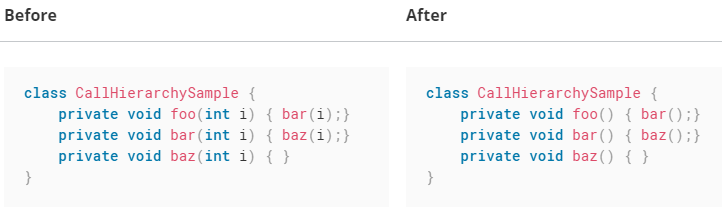
\includegraphics[scale=0.8]{Image/SafeDelete.png}\\
\itshape{Exemple de suppression sans  danger \cite{ref9}}
\end{center}

Par exemple on a une méthode "foo" avec un paramètre de type integer. Ce paramètre est ensuite passé à la méthode "bar" puis à la méthode "baz" où il est enfin utilisé.\\
Si on décide de supprimer le paramètre de la méthode "baz", l'IDE va, si demandé, effectuer le refactoring en supprimant le paramètre de toutes les méthodes puisqu'il n'était utilisé que dans la méthode "baz".
Cette option permet d'éviter d'avoir des oublis lorsqu'on supprime un élément et que l'on cherche où sont les répercussions.\\

\paragraph{Capacité de déplacement :}
L'IDE nous permet de déplacer des fonctionnalités à travers le code. On peut donc déplacer des méthodes ou des attributs vers d'autres classes si cela semble plus pertinent.\\

\paragraph{Extraction :}
On a aussi la possibilité d'effectuer des extractions de tous types, que ce soit pour extraire des méthodes, attributs ou paramètres (voir \textit{Extraction de méthode, Extraction de variable}).\\

\paragraph{Renommer :}
Et pour finir, il existe une fonctionnalité permettant de renommer n'importe quel élément. Cela nous permet de ne pas avoir à chercher dans le code toutes les occurrences de l'élément que l'on vient de modifier.\\

\subsection{Plugins}
Sur Eclipse et Intellij, il existe des plugins permettant de générer des graphes de flots de contrôle ou bien faire du refactoring.\\

Par exemple il existe le plugin "Unnecessary Code Detector" (UCDetector) qui permet entre autre de détecter du code mort.\\

En revanche il n'existe aucun plugin permettant de faire du refactoring à l'aide des graphes de flots de contrôle.\\
Mais dans un futur plus ou moins proche, il est possible qu'un plugin Eclipse nommé AutoRefactor soit disponible et arrive à faire du refactoring à l'aide des graphes de flots de contrôle.\\
AutoRefactor est actuellement disponible mais n'utilise pas encore les graphes de flots de contrôle.\\

\section{UCDetector}

UCDetector est un plugin Eclipse qui permet de détecter du code java inutilisé uniquement s'il s'agit de code de type "public"\cite{ref21}.
Il permet donc de trouver des classes, méthodes ou bien des champs qui ne sont utilisés nulle part.\\
UCDetector est capable de réduire la visibilité du code en proposant de changer la visibilité des méthodes ou autre à "protected", "default" ou bien "private" selon les différents cas.\\
Il est aussi possible de détecter si un champ ou une méthode peut être déclaré en "final".\\
En revanche il existe des cas où UCDetector peut se tromper(il ne s'agit que de suggestion)\cite{ref21} dans l'indication de code mort si le code est utilisé par :\\
- l'API Reflection\cite{ref21}.\\
- des Frameworks tels que Spring, Hibernate\cite{ref21}\\
- un autre code qui utilise notre API\\
- un jars dans notre workspace\cite{ref21}\\


\newpage

\section{AutoRefactor}
\subsection{Présentation du projet}
Le projet AutoRefactor a été lancé par Jean-Noël Rouvignac. Il a décidé de se lancer dans ce projet car il était fatigué de "devoir prendre trop de temps pour appliquer les mêmes nettoyages de code encore et encore". L'objectif de ce projet est de faciliter la maintenance, moderniser le code, rendre le code plus léger et compact ainsi qu'augmenter les performances des programmes. Rouvignac a commencé à travailler sur les expressions rationnelles pour retravailler toute la base du code, mais les faux positifs étaient trop nombreux.\cite{ref7} Il a ensuite créé un greffon Eclipse (AutoRefactor) qui utilise  l'API des Java Development Tools (Eclipse JDT) qui est l'API qu'Eclipse utilise pour faire du refactoring.\\
Une première release du produit est sortie le 22 mars 2015 et plus récemment est sortie la version 1.2 (30 juin 2018).\\

\subsection{Fonctionnement du programme}
Je vais maintenant vous présenter un algorithme simplifié du fonctionnement d'AutoRefactor\cite{ref7}.

Le développeur choisit les règles de refactoring à appliquer puis le greffon prend la liste des refactorings.

1) Le fichier Java à analyser est parsé et produit un arbre syntaxique abstrait.\\

2) Pour chaque refactoring :\\
\tabto{0.8cm} 1) Cherche des opportunités de refactoring en visitant l'arbre syntaxique abstrait.\\
\tabto{0.8cm} 2) Génère les réécritures de code lorsqu'une  opportunité de refactoring a été identifiée.\\

3) Lorsque tout l'arbre syntaxique abstrait a été visité, si des réécritures de code ont été générées :\\
\tabto{0.8cm} 1) Alors, toutes les réécritures de code générées sont appliquées sur le fichier.\\
\tabto{0.8cm} 2) Le fichier est sauvegardé.\\
\tabto{0.8cm} 3) Boucle vers 1.\\
\tabto{0.8cm} 4) Sinon, fin : il n'y a plus de refactoring possible sur ce fichier.\\

Actuellement, tous les refactorings implémentés font du filtrage par motif et travaillent fichier par fichier.\\

\newpage

\subsection{Fonctionnalités}
Il existe beaucoup de fonctionnalités de refactoring dans AutoRefactor; en voici quelques unes.\\

\paragraph{Remplacement de boucle par une seule méthode :}
AutoRefactor peut détecter des boucles inutiles liées à l'ajout ou à la suppression d'éléments dans des objets de type "List", "Map", "Collection".\\

\begin{center}
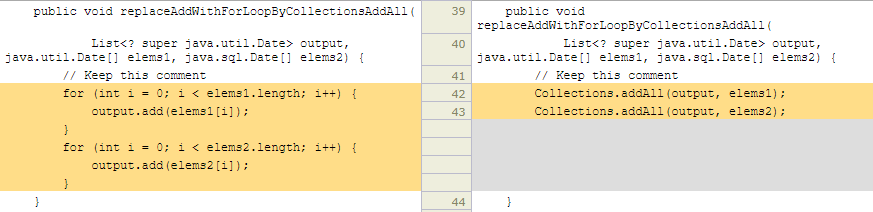
\includegraphics[scale=0.7]{Image/SupBoucle.png}\\
\itshape{Exemple de suppression de boucle \cite{ref10}}
\end{center}


On peut voir sur l'exemple ci-dessus que les boucles pour parcourir les listes ont été supprimées au profit d'une simple méthode.\\

\paragraph{Changement de type de stockage :}
Il existe des refactoring dans AutoRefactor qui modifient le type de variable pour en préférer d'autres.\\
Par exemple remplacer tous les types Vector et LinkedList par des ArrayList ou bien préférer des ArrayDeque à des Stack. Il en existe beaucoup d'autres à disposition.\\

\paragraph{Préférer les types primitifs :}
AutoRefactor nous permet de modifier le type de toutes les variables en un type primitif si cela est possible.\\
Par exemple si AutoRefactor détecte un objet de type Boolean, il va alors modifier le code pour utiliser le type boolean primitif. Cela peut être utilisé sur tous les types primitifs.\\

\paragraph{Fusionner les blocs if :}
On peut aussi détecter des blocs if qui peuvent s'emboiter pour n'en former plus qu'un.

\begin{center}
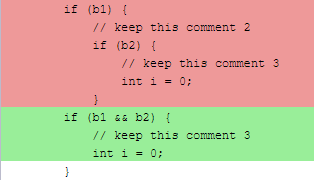
\includegraphics[scale=1]{Image/FusionIf.png}\\
\itshape{Exemple de fusion de bloc if \cite{ref10}}
\end{center}

\paragraph{Remplacer des clauses redondantes :}
AutoRefactor est capable de détécter des conditions inutiles qui peuvent être remplacées par une simple condition "or".

\begin{center}
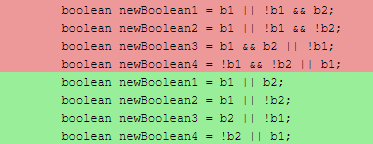
\includegraphics[scale=1]{Image/ClauseRedondante.png}\\
\itshape{Exemple de suppression de clause redondante\cite{ref10}}
\end{center}


\subsection{Objectif futur}
Jean-Noël Rouvignac a pour objectif futur de réussir à construire des graphes de flots de contrôle pour pouvoir les analyser. Ceci lui permettrait d'écrire des refactorings comprenant les chemins d'exécution du code, comme le ferait un développeur qui lirait du code. En particulier, il deviendrait possible de réduire la portée des variables, comprendre quels chemins d'exécution du code sont morts (impossibles à atteindre).\cite{ref7}\\
Il aimerait développer une fonctionnalité d'extraction automatique de méthode pour simplifier les longues méthodes.\\

\newpage

\section{Bilan}
Aujourd'hui, il n'existe aucun outil existant permettant de faire du refactoring à l'aide des graphes de flots de contrôle.\\
On retrouve énormément d'outils permettant de générer des graphes de flots de contrôle afin de pouvoir mieux visualiser le fonctionnement de son programme.\\
On trouve aussi des plugins ou bien des projets qui permettent de faire du refactoring notamment AutoRefactor qui est le seul logiciel de refactoring existant avec l'ambition d'utiliser les graphes de flots de contrôle dans le refactoring.\\ 

\chapter{Conclusion}
Nous avons pu constater que tous nos programmes peuvent rapidement être infestés de codes mal structurés ou d'éléments indésirables.\\
On a pu voir qu'il existe de nombreuses manières de faire du refactoring pour augmenter la lisibilité du code, réduire sa taille en supprimant les doublons ou tout simplement augmenter la qualité du code.\\
Puis nous avons vu des outils permettant de faire du refactoring.\\
Il y a les IDE tel que IntelliJ ou bien Eclipse qui proposent des possibilités de refactoring basique.\\
Ensuite nous avons regardé AutoRefactor un outil en cours de développement qui utilise actuellement le filtrage par motif pour effectuer du refactoring et qui par la suite aimerait utiliser les graphes de flots de contrôle.\\
Et pour finir nous avons étudié les graphes de flots de contrôle ainsi que l'exécution symbolique et nous nous sommes rendu compte qu'il était théoriquement possible de les utiliser pour faire du refactoring.\\
En conclusion, le refactoring est un remaniement du code très important car il ne faut pas se reposer sur des ordinateurs ultra puissants pour produire du code de très mauvaise qualité. Le refactoring permet aussi de rendre le code plus compréhensible et plus facile à maintenir donc de réduire les coûts de développement.
Le refactoring doit être appliqué à bon escient selon le contexte.\\
Et à l'avenir je pense qu'il serait intéressant de se pencher sur les graphes de flots de contrôle pour les utiliser dans certaines parties du refactoring telle que la détection de code mort.\\


\bibliographystyle{plain}
\bibliography{bibliographie}
\end{document}
